\bigskip
\bigskip
\subsubsection*{Խնդիրներ և հարցեր թեմա 7-ի վերաբերյալ}

\begin{enumerate}[label=\thesection.\arabic*.]
% 7.1 
\item Ապացուցեք, որ $$\rho : \R \times \R \to \R, \qquad \rho(x,y)=(x-y)^2$$ արտապատկերումը չի որոշում մետրիկ $\R$ թվային ուղղի վրա։ 

% 7.2
\item Ցույց տվեք, որ $n>1$ դեպքերում 
\[
\rho: \R^n \times \R^n \to \R, \qquad \rho(x, y ) = \min_{1\le i \le n} |x_i-y_i|,
\]
\[
x=(x_1, x_2, \dots, x_n),\qquad y=(y_1, y_2, \dots, y_n)
\] 
արտապատկերումը չի որոշում մետրիկ $\R^n$-ում։

% 7.3
\item Ապացուցեք․ $X$ բազմության վրա մետրիկի 1-3 աքսիոմները համարժեք են հետևյալ 
երկու աքսիոմներին՝
\begin{enumerate}
\item[1.] $\rho(x,y)=0$ այն և միայն այն դեպքում, երբ $x=y$,
\item[2.] $\rho(x,y) \le \rho(z,x)+\rho(z,y)$ բոլոր $x, y, z \in X$ տարրերի դեպքում։
\end{enumerate}


% 7.4
\item Ապացուցեք․ եթե $\rho$-ն որևէ մետրիկ է $X$ բազմության վրա, ապա 
\[
\tilde{\rho} : X \times X \to \R,
\qquad 
\tilde{\rho}(x,y) = \min\left(1, \rho(x,y)\right)
\]
արտապատկերումը նույնպես մետրիկ է $X$-ի վրա։ 

% 7.5
\item Ցույց տվեք, որ $X$ բազմության վրա նախորդ խնդրում դիտարկված $\rho$ և $\tilde{\rho}$ մետրիկները համարժեք են (որոշում են $X$-ի միևնույն տոպոլոգիան):

% 7.6
\item Գտեք այնպիսի մետրիկային տարածություն և նրանում երկու այնպիսի փակ գնդեր, որ դրանցից ավելի մեծ շառավղով գունդը պարունակվի ավելի փոքր շառավղով գնդի մեջ՝ չհամընկնելով նրա հետ։

% 7.7
\item Դիտարկենք $\R^2$ կոորդինատային հարթությունը և
\[
\sigma: \R^2 \times \R^2 \to \R, \qquad \sigma(x, y ) = |x_1-y_1|+|x_2-y_2|, \qquad
x=(x_1, x_2),\ y=(y_1, y_2)
\]
արտապատկերումը:
\begin{enumerate}
\item[ա)] Ապացուցեք, որ $\sigma$-ն որոշում է մետրիկ $\R^2$-ի վրա։

\item[բ)] Նկարագրեք ստացվող մետրիկային տոպոլոգիայի կանոնական բազան։
\end{enumerate}

\par \textbf{Ցուցում} բ)-ի վերաբերյալ․ Սևեռված $x^0 = (x_1^0, x_2^0)$ կետի դեպքում՝ $\mathcal{D}(x^0, r) = \{y \in \R^2 : |x_1^0-y_1|+|x_2^0-y_2|<r\}$։ Մասնավորապես $x^0=O=(0,0)$ կետի դեպքում $\mathcal{D}(0, r) = \{y\in\R^2 : |y_1|+|y_2|<r\}$ բաց շրջանը անեզր քառակուսի է, որի կենտրոնը կոորդինատների սկզբնակետն է, իսկ $2r$ երկարությամբ անկյունագծերը գտնվում են կոորդինատային առանցքների վրա։ Ցույց տվեք, որ ընդհանուր դեպքում $\mathcal{D}(x^0, r)$ շրջանը ստացվում է $\mathcal{D}(O, r)$ քառակուսուց՝ նրա $O$ կենտրոնի զուգահեռ տեղափոխությունով $x^0$ կետ։

\begin{center}
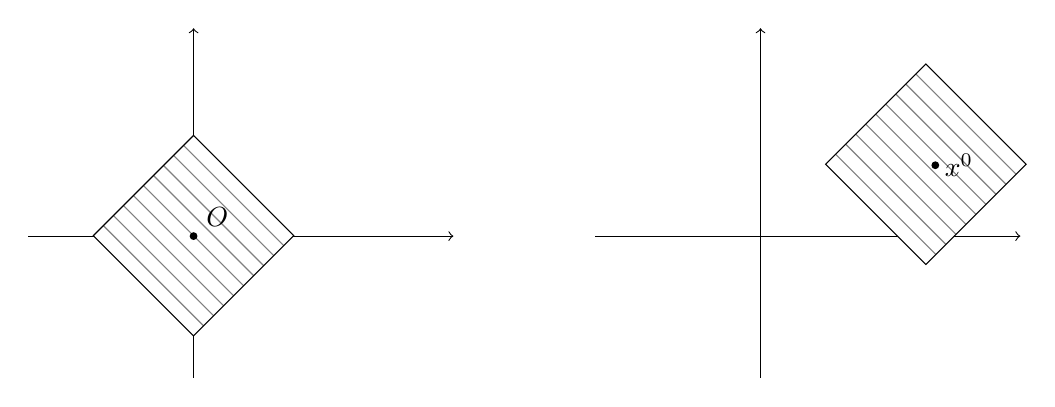
\begin{tikzpicture}[scale=1.2]

% Left diamond
\draw[->] (-3,0) -- (1.5,0); % x-axis
\draw[->] (-1.25,-1.5) -- (-1.25,2.2); % y-axis

\begin{scope}[shift={(-1.25,-0.704*1.5)}, rotate=45]
    \draw[fill=white] (0,0) rectangle (1.5,1.5);
    \foreach \x in {0.15,0.3,...,1.5}
        \draw[opacity=0.5] (\x,0) -- (\x,1.5);
\end{scope}
% Mark center and theta
\node at (-1.25,0) [circle,fill=black,inner sep=1pt]{};
\node at (-1.0,0.2) {$O$};

\begin{scope}[shift={(1.5,0)}]


% Right diamond
\draw[->] (1.5,0) -- (6,0); % x-axis
\draw[->] (3.25,-1.5) -- (3.25,2.2); % y-axis
\begin{scope}[shift={(5,-0.3)}, rotate=45]
    \draw[fill=white] (0,0) rectangle (1.5,1.5);
    \foreach \x in {0.15,0.3,...,1.5}
        \draw[opacity=0.5] (\x,0) -- (\x,1.5);
\end{scope}
% Mark center and points
\node at (5.1,0.75) [circle,fill=black,inner sep=1pt]{};
% \node at (3.55,0.3) {$0$};
\node at (5.35,0.75) {$x^0$};
\end{scope}
\end{tikzpicture}
\end{center}


% 7.8
\item Լուծեք նախորդ խնդիրը
\[
\mu : \R^2 \times \R^2 \to \R, 
\qquad 
\mu(x, y) = \max\left\{ |x_1-y_1| + |x_2-y_2| \right\}
= \max_{i=1, 2} |x_i-y_i| 
\]
արտապատկերման դեպքում, որտեղ $x=(x_1,x_2)$, $y=(y_1, y_2)$:


\begin{center}
\begin{tikzpicture}[scale=1.2]

% Left diamond
\draw[->] (-3,0) -- (1.5,0); % x-axis
\draw[->] (-1.25,-1.5) -- (-1.25,2.2); % y-axis

\begin{scope}[shift={(-2,-1.5/2)}, ]
    \draw[fill=white] (0,0) rectangle (1.5,1.5);
    \foreach \x in {0.15,0.3,...,1.5}
        \draw[opacity=0.5] (\x,0) -- (\x,1.5);
\end{scope}
% Mark center and theta
\node at (-1.25,0) [circle,fill=black,inner sep=1pt]{};
\node at (-1.0,0.2) {$O$};

\begin{scope}[shift={(1.5,0)}]


% Right diamond
\draw[->] (1.5,0) -- (6,0); % x-axis
\draw[->] (3.25,-1.5) -- (3.25,2.2); % y-axis
\begin{scope}[shift={(5.1-1.5/2-0.2,0.75-1.5/2-0.2)}]
    \draw[fill=white] (0,0) rectangle (1.5,1.5);
    \foreach \x in {0.15,0.3,...,1.5}
        \draw[opacity=0.5] (\x,0) -- (\x,1.5);
\end{scope}
% Mark center and points
\node at (5.1-0.2,0.75-0.2) [circle,fill=black,inner sep=1pt]{};
% \node at (3.55,0.3) {$0$};
\node at (5.35-0.2,0.75-0.2) {$x^0$};
\end{scope}
\end{tikzpicture}
\end{center}


\par \textbf{Ցուցում} բ)-ի վերաբերյալ․ Ցույց տվեք, որ սևեռված $x^0 = (x_1^0, x_2^0)$ կետի դեպ\-քում $x^0$ կենտրոնով, $r$ շառավղով $\mathcal{D}(x^0, r) = \{y \in \R^2 : \mu(x^0 , y)<r\}$ բաց շրջանը ստացվում է $O=(0, 0)$ կենտրոնով և $2r$ կողմով $\mathcal{D}(O, r) = \{y \in \R^2 : |y_1|<r,\ |y_2|<r\}$ անեզր քառակուսուց՝ նրա $O$ կենտրոնի զուգահեռ տեղափոխությունով $x^0$ կետ։

% 7.9
\item Ապացուցեք, որ 7.7 և 7.8 խնդիրներում սահմանված $\sigma$ և $\mu$ մետրիկները համ\-ար\-ժեք են (որոշում են $\R^2$-ի նույն տոպոլոգիան)։

% 7.10
\item Երկրաչափորեն նկարագրեք՝ ինչ են պրոյեկտիվ հարթության մետրիկային տոպոլոգիայի կանոնական բազայի տարրերը։ 

\begin{hint} Սևեռելով $\R^3$-ում $O$ սկզբնակետով անցնող որևէ $l^0$ ուղիղ և որևէ $\alpha$ սուր անկյուն՝ դիտարկեք $O$ կետով անցնող բոլոր $l$ ուղիղների բազմությունը, որոնք $l^0$ ուղղի հետ կազմում են $\alpha$-ն չգերազանցող անկյուն։ Պարզեք, թե այդ անեզր գնդի համար երկրորդ կարգի ո՞ր մակերևույթն է հանդիսանում եզրային սֆերա։ 
\end{hint}


% 7.11
\item Դիտարկենք $\R^n$, $n \ge 1$ կոորդինատային տարածությունը \hyperref[օրինակ 3]{օրինակ 3}-ում \linebreak սահ\-մանված $\rho(x,y) = \sqrt{(x_1-y_1)^2+(x_2-y_2)^2+\dots+(x_n-y_n)^2}$ մետրիկով։ Ապացուցեք, որ այդ մետրիկային տարածությունում ամեն մի $\mathcal{S}(a, r)$ սֆերա հանդիսանում է տվյալ $\mathcal{D}(a, r)$ գնդի եզր՝ ըստ թեմա 6-ում սահմանված ենթա\-բազմության եզր հասկացության։

\end{enumerate}
